\documentclass{article}

% If you're new to LaTeX, here's some short tutorials:
% https://www.overleaf.com/learn/latex/Learn_LaTeX_in_30_minutes
% https://en.wikibooks.org/wiki/LaTeX/Basics

\def\rd{{\rm d}}
\def\ds{\displaystyle}

% Formatting
\usepackage[utf8]{inputenc}
\usepackage[margin=1in]{geometry}
\usepackage[titletoc,title]{appendix}
\usepackage{amsmath} 
% Math
% https://www.overleaf.com/learn/latex/Mathematical_expressions
% https://en.wikibooks.org/wiki/LaTeX/Mathematics
\usepackage{amsmath,amsfonts,amssymb,mathtools}

% Images
% https://www.overleaf.com/learn/latex/Inserting_Images
% https://en.wikibooks.org/wiki/LaTeX/Floats,_Figures_and_Captions
\usepackage{graphicx,float}

% Tables
% https://www.overleaf.com/learn/latex/Tables
% https://en.wikibooks.org/wiki/LaTeX/Tables

% Algorithms
% https://www.overleaf.com/learn/latex/algorithms
% https://en.wikibooks.org/wiki/LaTeX/Algorithms
\usepackage[ruled,vlined]{algorithm2e}
\usepackage{algorithmic}

% Code syntax highlighting
% https://www.overleaf.com/learn/latex/Code_Highlighting_with_minted
\usepackage{minted}
\usemintedstyle{borland}

% References
% https://www.overleaf.com/learn/latex/Bibliography_management_in_LaTeX
% https://en.wikibooks.org/wiki/LaTeX/Bibliography_Management
\usepackage{biblatex}
\addbibresource{references.bib}

% Title content
\title{AMATH 482 Homework 5}
\author{Yiping Li}
\date{March 17, 2021}

\begin{document}

\maketitle

% Abstract
\begin{abstract}
    In this study, we are asked to separate the video stream to both the foreground video and a background, using the Dynamic Mode Decomposition method (DMD).
\end{abstract}

% Introduction and Overview
\section{Introduction and Overview}
% Example Subsection
\subsection{Problem Setting}
The first video contains several running Formula 1 cars and one waving flag. The background is almost the same at every frame except that the camera was slightly shaking. The second video contains a person skiing down from a mountain. Again, our task is to separate the foreground and the background video. In other words, we need to extract the motion out of the background.
% Example Subsubsection
\subsection{Data Format}
All video inputs are given in \texttt{MP4} file. The first video is about 6 seconds long and has the resolution of 1872 * 1112. Its frame per second (fps) is around 60. The second video is about 7 seconds long and has the resolution of 1466 * 1604. Its fps is also around 60. Notice that for each frame we need to store 2 million numbers and each video has over 300 frames, which give us around 600 million numbers. We tried to process those original videos, but it turns that the memory of our device is not enough to hold such amount of data. Thus, we used the videos with lower resolution (960 * 540).
%  Theoretical Background
\section{Theoretical Background}
The most significant trait of DMD is that it linearizes non-linear things. Suppose $U(x_i, t_j)$ describes the state of the $i^{th}$ element at time $t_j$, if we use rows to code elements and columns to code time, we would get a matrix $\mathbf{X}$ such that,
\[
\mathbf{X} = 
\begin{bmatrix}
U(x_1, t_1) & U(x_1, t_2) & \dots & U(x_1, t_M) \\
U(x_2, t_1) & U(x_2, t_2) & \dots & U(x_2, t_M) \\
\vdots & \dots & \ddots & \vdots \\
U(x_N, t_1) & U(x_N, t_2) & \dots & U(x_N, t_M) \\
\end{bmatrix}
\]
Now, let 
\[
\mathbf{X_{jk}} = 
\begin{bmatrix}
U(\mathbf{x}, t_j) & U(\mathbf{x}, t_{j+1}) & \dots & U(x_1, t_k) \\
\end{bmatrix}
\]
The DMD method approximates the modes of the Koopman operator, which is a linear, time-independent operator that
\[
\mathbf{X}_{j+1} = \mathbf{AX}_j
\]
Find such linear operator allowed us to predict states at any time, but the actual valid prediction range is bounded. \\
~\\
To do such decomposition, we find matrices $\mathbf{X_1}$ and $\mathbf{X_2}$ such that,
\[
\mathbf{X_1}=\mathbf{X_1^{M-1}} = [\mathbf{x_1},\mathbf{x_2},\dots, \mathbf{x_{M-1}}] = [\mathbf{x_1},\mathbf{Ax_1},\dots, \mathbf{A^{M-2}x_{1}}]
\]
\[
\mathbf{X_2}=\mathbf{X_2^{M}} = [\mathbf{x_2},\mathbf{x_3},\dots, \mathbf{x_{k}}]= [\mathbf{Ax_1},\mathbf{A^2x_1},\dots, \mathbf{A^{M-1}x_{1}}]
\]
Therefore, we can rewrite $\mathbf{X_2}$ as
\[
\mathbf{X_2} = \mathbf{AX_1} + \mathbf{r}e^T_{M-1}.
\]
where the second term is the error of $\mathbf{x_M}$ since it is not include in the Krylox space of $\mathbf{X_1}$. \\
~\\
Again, our goal is to find the operator $\mathbf{A}$, therefore let's apply SVD on  $\mathbf{X_1}$, and we have
\[
\mathbf{X_2} = \mathbf{AU\Sigma V^*} + \mathbf{r}e^T_{M-1}.
\]
Now, we are going to find $\mathbf{A}$ when $\mathbf{X_2}$ is projected to the space with the basis of $\mathbf{U}$. In other words, we want to find the matrix $\mathbf{A}$ in the POD modes. Therefore, the error must be orthogonal to the POD basis, which leads to $\mathbf{U^*r=0}$.
\[
\mathbf{U^*X_2} = \mathbf{U^*AU\Sigma V^*}.
\]
By moving variables around, the final equation will be
\[
\mathbf{U^*AU} = \mathbf{U^*X_2\Sigma V^*=\tilde{S}}.
\]
Next, suppose $\mathbf{y_k}$ and $\mu_k$ are the eigen vector and eigenvalues of $\mathbf{\tilde{S}}$. Therefore, 
\begin{equation}
    \begin{aligned}
    \mathbf{\tilde{S}y_k} &= \mu_k \mathbf{y_k} \\
    \mathbf{U^*AUy_k} &=  \mu_k \mathbf{y_k} \\
    \mathbf{AUy_k} &=  \mu_k \mathbf{Uy_k} \\
    \end{aligned}
\end{equation}
The computation above shows that the eigen vector of $\mathbf{A}$ us $\mathbf{Uy_k}$, which is also the DMD modes $\phi_k$. The continues multiplication of matrix $\mathbf{A}$ can be given by expanding it in eigen basis, thus the prediction model is described as
\[
\mathbf{X_{DMD}(t)} = \sum_{k=1}^K b_k \phi_k e^{w_k t} = \Phi \textbf{diag} (e^{w_k t}) \mathbf{b},
\]
where $e^{w_k t}$ is just another way to write the eigenvalues $\mu_k$, and the matrix $b$ is the initial condition, which is given by $\Phi^\dagger x_i$, and $x_i$ is the initial state we want to start with.
% Algorithm Implementation and Development
\section{Algorithm Implementation and Development}
\subsection{Preparation}
Since the videos are provided in \texttt{MP4} format, we have to load the videos and reshape it before we actually apply the algorithm.
\begin{algorithm}
\begin{algorithmic}
    \STATE{Load the video by \texttt{VideoReader}}
    \STATE{Store information including total frame number, fps, frame height, and frame width}
    \FOR{each frame}
        \STATE{Turn the frame into gray-scale image}
        \STATE{Flat the matrix into a vector, which will be $\mathbf{X_i}$}
    \ENDFOR
\end{algorithmic}
\caption{Preparation}
\end{algorithm}


\subsection{Finding the low-rank reconstruction and applying the DMD.}
Notice that in the DMD, there is a step which we need to apply the SVM on $\mathbf{X_1}$. By doing this, we are able to find the principle components of the frame at each time $t_i$. Remember that, the component with the heaviest weight is the one shared in all frames! Therefore, if we select some heavy components, we are probably going to capture the background of the video.
\newpage
\begin{algorithm}
\begin{algorithmic}
    \STATE{...(normal DMD procedure)}
    \STATE{Apply the SVM on $\mathbf{X_1}$}
    \STATE{Select first $n$ components for reconstruction, and find the corresponding $\mathbf{U,\Sigma,V} $}
    \STATE{...(normal DMD procedure)}
\end{algorithmic}
\caption{Finding the low-rank reconstruction and applying the DMD.}
\end{algorithm}

\subsection{Finding the background and the foreground}
Since the DMD reconstruction gives us complex numbers, therefore we have to do moves to get a clear data of the background and the foreground.
\begin{algorithm}
\begin{algorithmic}
    \STATE{Find $\mathbf{X_{sparse}}$ by $\mathbf{X1}-|\mathbf{X_{DMD}^{low-rank}}|$}
    \STATE{Find the real part $\mathbf{R}$ of $\mathbf{X_{sparse}}$}
    \STATE{Find the background by $\mathbf{R} + |\mathbf{X_{DMD}^{low-rank}}|$}
    \STATE{Find the foreground by $\mathbf{X_{sparse}} - \mathbf{R}$}
\end{algorithmic}
\caption{Finding the background and the foreground}
\end{algorithm}

\section{Computational Result}
Here are some examples of the separation.
\subsection{monte\_carlo\_low.mp4}
\begin{figure}[h]
    \centerline{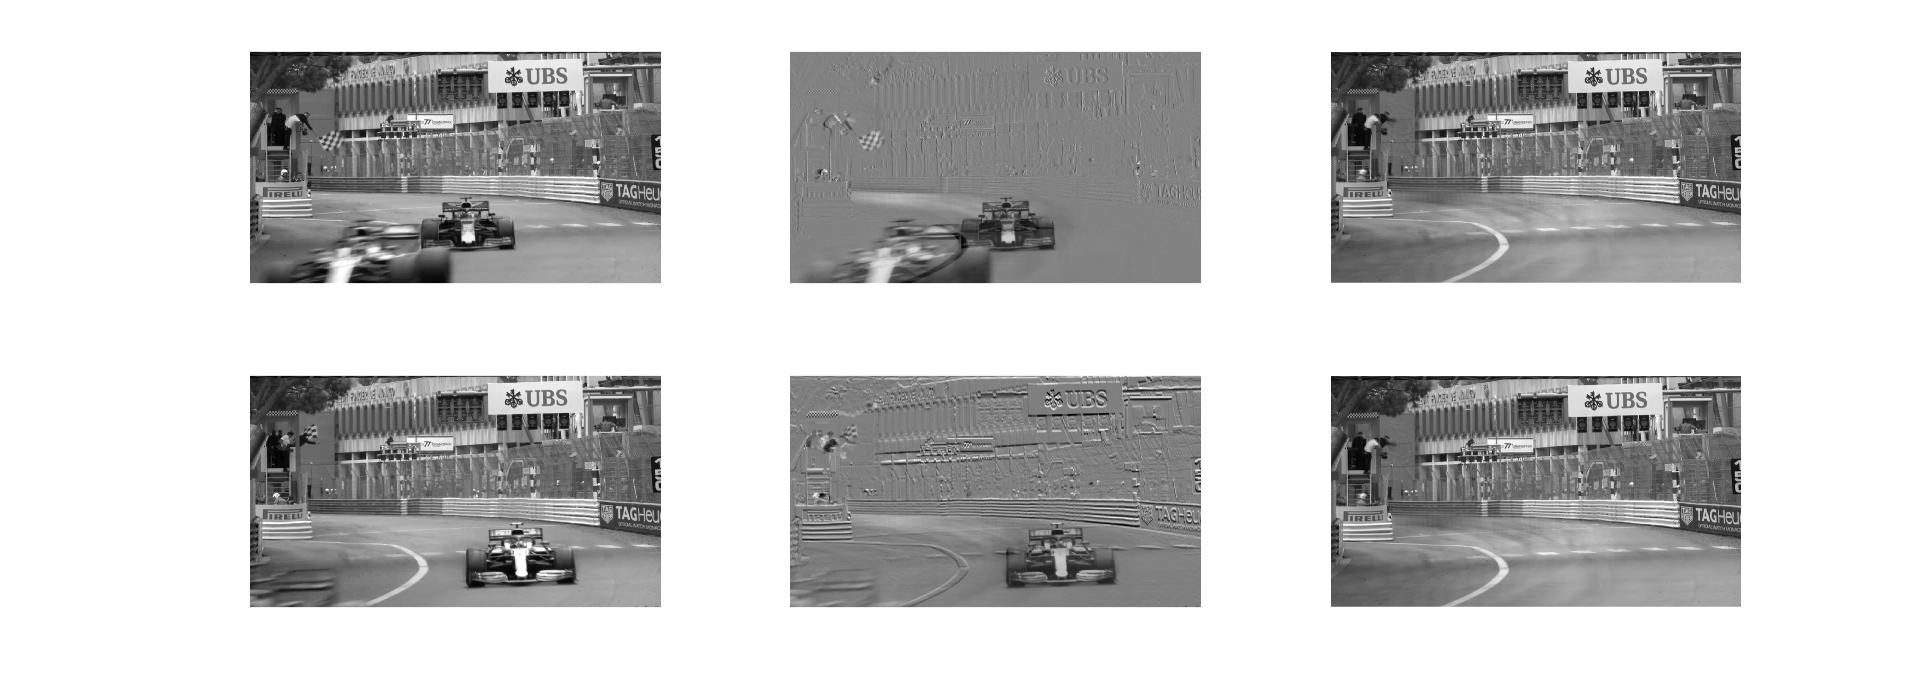
\includegraphics[width=7in]{f1.jpg}}
    \caption{Original (left), Foreground (middle), and Background (right)}
\end{figure}

Here are extractions of the foreground and the background
\subsection{ski\_drop\_low.mp4}
\begin{figure}[h]
    \centerline{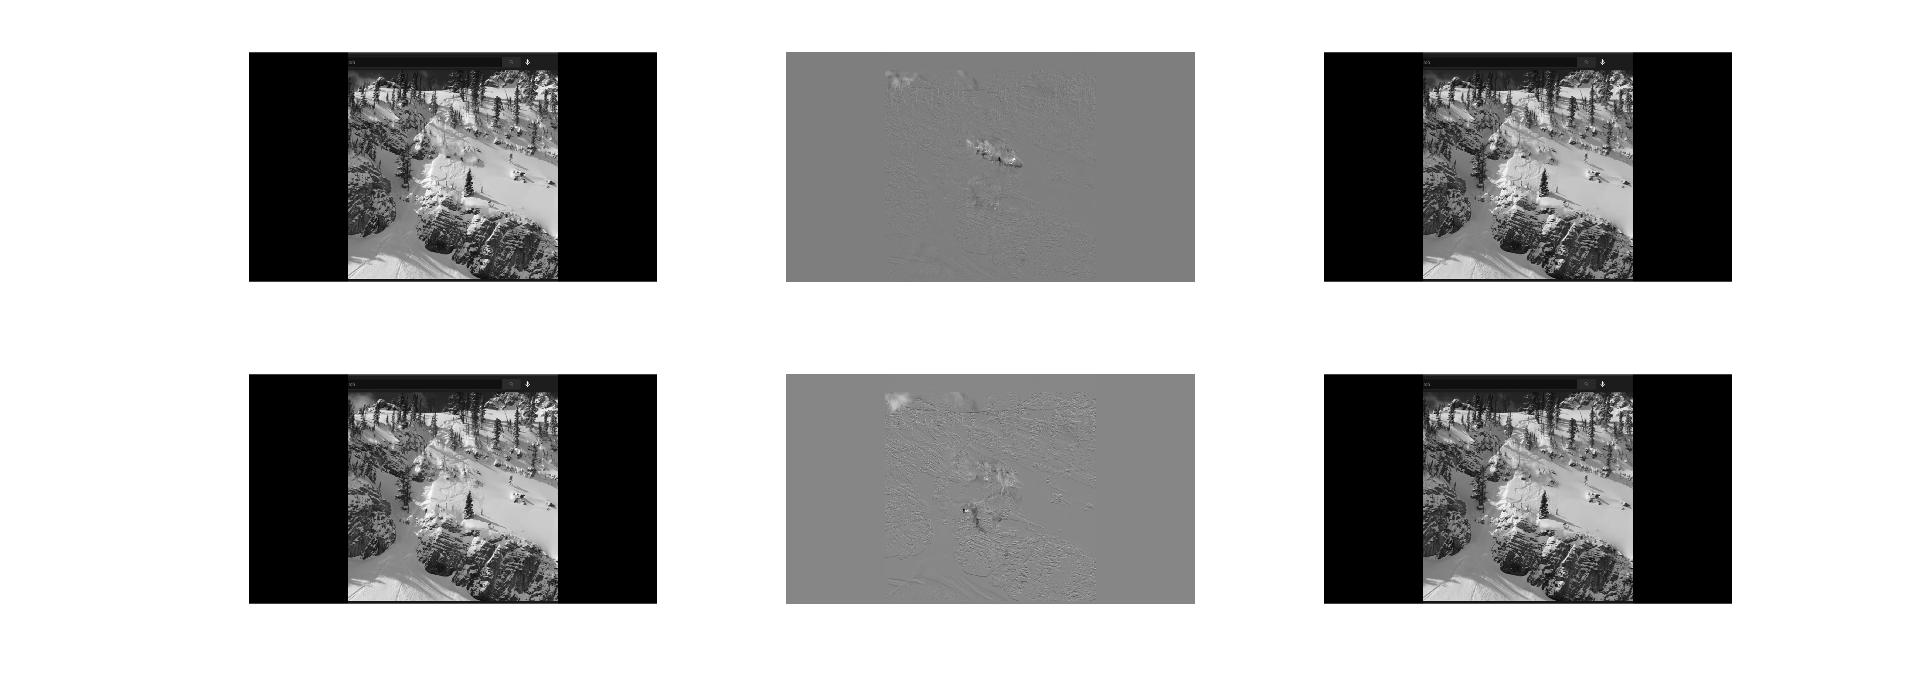
\includegraphics[width=7in]{ski.jpg}}
    \caption{Original (left), Foreground (middle), and Background (right)}
\end{figure}

\section{Summary and Conclusion}
In the study, we successfully separated the foreground and the background of two videos by applying the DMD and SVM. The SVM is always a powerful tool for breaking down something to see its components.
~\\
% Appendices
\begin{appendices}


% MATLAB Codes

\section{MATLAB Code}

\begin{verbatim}
%% clear all
clear all; close all; clc;

%% Setup
X = get_video('ski_drop_low.mp4');
dt = 60;
t = linspace(0,size(X,2)/dt, size(X,2)-1);

%% Create DMD matrices

X1 = X(:,1:end-1);
X2 = X(:,2:end);

%% SVD of X1 and Computation of ~S

[U, Sigma, V] = svd(X1,'econ');

rank = 10;
U_l = U(:, 1:rank); % truncate to rank-r
Sigma_l = Sigma(1:rank, 1:rank);
V_l = V(:, 1:rank);
S = U_l'*X2*V_l*diag(1./diag(Sigma_l));
[eV, D] = eig(S); % compute eigenvalues + eigenvectors
mu = diag(D); % extract eigenvalues
omega = log(mu)/dt;
Phi = U_l*eV;

%% Create DMD Solution

b = Phi\X1(:,1); % pseudoinverse to get initial conditions

u_modes = zeros(length(b),length(t));
for iter = 1:length(t)
   u_modes(:,iter) = b.*exp(omega*t(iter)); 
end
u_dmd = Phi*u_modes;

%% Create Sparse and Low-Rank

Xsparse = X1 - abs(u_dmd);
clear X1; clear X2; clear U;
R = zeros(length(Xsparse), size(Xsparse, 2));

X_bg = R + abs(u_dmd);
X_fg = Xsparse - R;



%% Generate plots
frame = [80, 240];

for i=1:2
    org = imresize(rescale(reshape(X(:,frame(i)), 540, 960)),2);
    fg = imresize(rescale(reshape(X_fg(:,frame(i)), 540, 960)),2);
    bg = imresize(rescale(reshape(X_bg(:,frame(i)), 540, 960)),2);
    subplot(2,3,3*i-2);
    imshow(org);
    subplot(2,3,3*i-1);
    imshow(fg);
    subplot(2,3,3*i);
    imshow(bg);
end




function mat = get_video(video_name)
obj = VideoReader(video_name);
vid = read(obj);
frames = obj.NumberOfFrames;
mat = [];
for x = 1 : frames
    frame = vid(:,:,:,x);
    frame = rgb2gray(frame);
    frame = double(frame(:));
    mat = [mat, frame];
end


end

\end{verbatim}


\end{appendices}

\end{document}
